\chapter{Diseño del sistema}
\label{chap:disenosistema}
En este capítulo se describirá el diseño del sistema desarrollado. 
En la sección 3.1 se detallará la arquitectura del sistema global. 
En el apartado 3.2 se profundizará en la arquitectura interna del HUB.
\lsection{Necesidades del sistema}
En esta sección se analizarán las necesidades de nuestro sistema y los dispositivos con los que nos comunicaremos.
\subsection{Necesidades de los dispositivos}
Antes de empezar a diseñar el sistema y elegir el protocolo que se utilizará y el medio físico por el que se comunicarán 
nuestros dispositivos es necesario analizar los dispositivos que podrán conectarse a nuestro HUB así como sus necesidades. 
Una vez determinados los requisitos del protocolo se estudiará el medio físico de comunicación.
\newline
\newline
Los principales dispositivos domóticos que hemos encontrado son: sensores de temperatura, sensores de humedad, 
sensores de luz, sensores de movimiento, medidores de distancia, sensores de humo, sensores magnéticos, cámaras, 
bombillas, enchufes, termostatos, motores, aires acondicionados, interruptores y altavoces.
\newline
Estos dispositivos pueden ser divididos en dos grupos: sensores y actuadores. 
\newline
Los sensores solamente envían determinada información a nuestro HUB (comunicación unidireccional), 
mientras que los actuadores reciben mensajes con determinados comandos a parte de enviar información del estado 
en el que se encuentran (comunicación bidireccional).

Agrupación de los dispositivos encontrados:

\begin{figure}[H]
\centering
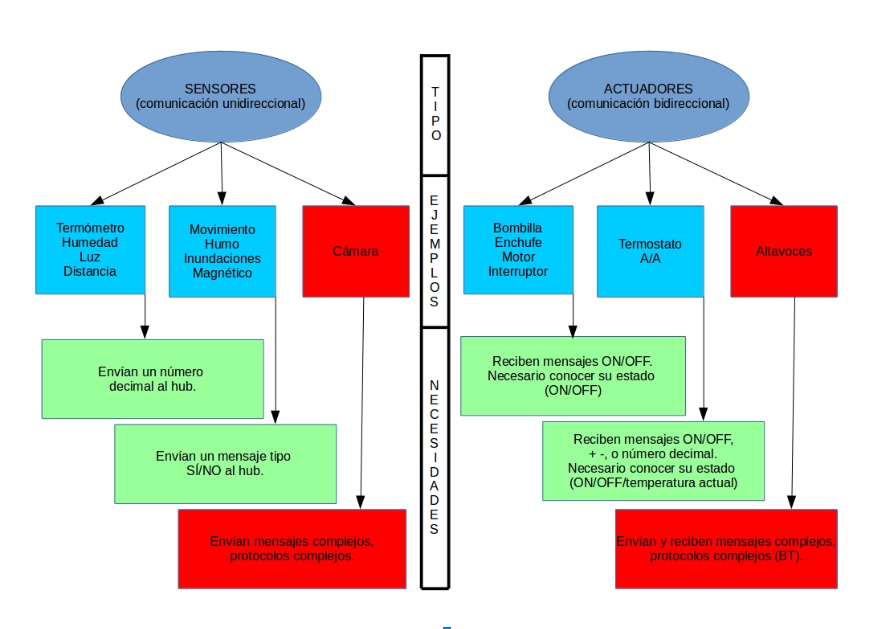
\includegraphics[width=6.00in]{images/descripcion_dispositivos.png}
\caption{Tipos de dispositivos}
\label{fig:descripcion_dispositivos}
\end{figure}


Para la definición del protocolo dividiremos los dispositivos en tres tipos:
\begin{itemize}
\item Tipo 1 (sensores): el hub sólo recibe información de los sensores. El hub no necesita saber qué tipo de información recoge (número decimal, SÍ/NO...etc), simplemente la actualiza y la muestra al usuario.
\item Tipo 2 (actuadores): estos dispositivos envían información al HUB y son capaces de recibir comandos tipo ON/OFF, +/-, número decimal...etc.
\item Tipo 3: cámaras IP. Este sensor recibirá un tratamiento especial debido a la necesidad de una comunicación constante y rápida.
\end{itemize}
\subsection{Necesidades del sistema}
Una vez analizadas las necesidades de los dispositivos podemos analizar las necesidades de nuestro sistema.
Para el desarrollo de nuestro sistema necesitaremos una arquitectura que nos permita:
\begin{itemize}
\item Comunicación bidireccional entre los dispositivos y el hub: es necesario que el hub conozca información de los dispositivos, 
registre dispositivos y gestione dispositivos, así como también es necesario que los dispositivos puedan recibir comandos provenientes
del hub. El hub debe permitir aceptar dispositivos con diferentes comandos, y no ceñirse sólo a un número cerrado de comandos (ON/OFF, +/-,...).
\item Comunicación entre el hub y la interfaz: será necesario que la información de los dispositivos y el estado de los mismos sea accesible
a través de la interfaz de usuario. Además el usuario debe ser capaz de gestionar los dispositivos y enviar comandos a los actuadores
a través de la interfaz.
\item Seguridad en la comunicación: es imprescindible que toda comunicación se realice de manera segura, de tal manera que nadie pueda modificar o
acceder a nuestra información.
\item Escalabilidad: aunque durante la realización de nuestro proyecto nos centraremos únicamente en la comunicación mediante protocolo HTTPS, 
es necesario diseñar un sistema escalable que el día de mañana pueda funcionar con diferentes protocolos y dispositivos.
\end{itemize}
\lsection{Protocolos}
En esta sección se describirá el protocolo que se utilizará en las comunicaciones entre los dispositivos y el HUB.
\subsection{Protocolo HTTPS}
El protocolo elegido para la comunicación entre dispositivos, hub e interfaz es el protocolo HTTPS (Hypertext Transfer Protocol Secure).
\newline
Este protocolo nos da la posibilidad de implementar una API REST consumible por parte de los dispositivos y por parte de la interfaz,
sin necesidad de utilizar diferentes protocolos para los diferentes canales.
\newline
Además, de estar muy estandarizadas a día de hoy, las APIs REST nos dan la capacidad de separar entre cliente y servidor y de ser capaces
de utilizar diferentes lenguajes y tecnologías para cada lado. Es decir, podemos tener un servidor escrito en Express.js (javascript), una interfaz 
gráfica utilizando Angular5 (TypeScript), y unos actuadores/sensores que utilicen CherryPy (Python).
\newline
Además, utilizar HTTPS nos ofrece la posibilidad de crear un canal de comunicación cifrado, de manera que la información que circula en dicho 
canal no pueda ser descifrada por ningún intermediario ni se pueda sufrir un ataque Man-In-The-Middle*.
\lsection{Arquitectura del sistema}
En esta sección se describirá el diseño y la arquitectura del sistema de manera global, incluyendo dispositivos actuadores, 
dispositivos sensores y el propio hub.
\subsection{Arquitectura del sistema}
Teniendo en cuenta las necesidades de nuestro sistema realizaremos una arquitectura similar a las arquitecturas de microservicios,
en la que el hub y los actuadores serán los hosts de un servidor REST y serán capaces de recibir y procesar peticiones.
\newline
El hub recibirá peticiones de parte de la interfaz de usuario y de los dispositivos, y lanzará peticiones a los actuadores.
Para ello se establecerán dos APIS publicadas por el HUB y consumibles por la interfaz de usuario y los dispositivos:
\begin{itemize}
\item \underline{Interface API:} será consumida por la interfaz de usuario. Se encargará de enviar la información de los dispositivos al usuario: número
 de dispositivos, localización, etc... Además, permitirá al usuario gestionar dispositivos y enviarles comandos.
\item \underline{Sensors API:} será consumida por actuadores y sensores por igual. Permitirá a los dispositivos darse de alta en el sistema y actualizar
periódicamente su información.
\end{itemize}
Los actuadores, además de lanzar peticiones al hub para informar de su estado, deberán ser capaces de recibir peticiones del hub con
diferentes comandos. Para ello se establecerá otra API que todos los dispositivos deberán seguir, para que así el HUB consuma la misma API
en los diferentes dispositivos. Será denominada en adelante como \underline{Actuators API}.
\newline
Estableceremos y explicaremos estas APIs en los capítulos siguientes.
\newline
Todas las peticiones deben ser securizadas, y debemos asegurar que ningún intruso pueda acceder y/o modificar la información de nuestro sistema.

Esquema de la arquitecura a seguir:
\begin{figure}[H]
\centering
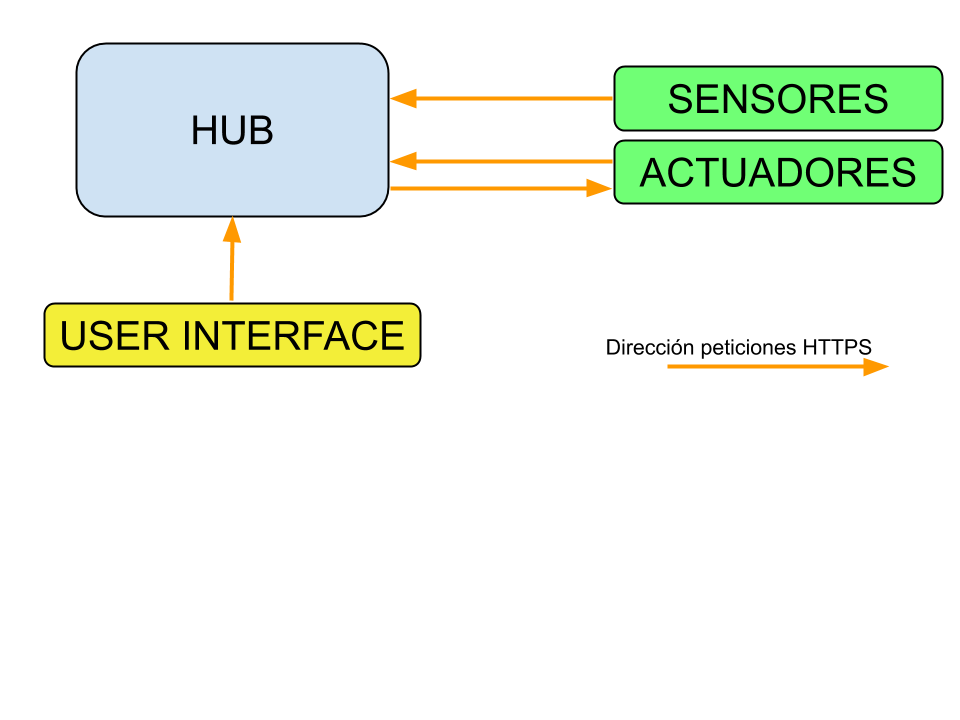
\includegraphics[width=6.00in]{images/esquema_arquitectura.png}
\caption{Tipos de dispositivos}
\label{fig:descripcion_dispositivos}
\end{figure}

\subsection{Modelo de datos}
En esta sección se describirán los modelos de datos a utilizar. Todos los datos residirán en el HUB, que será el encargado de orquestarlos,
organizarlos y mantenerlos.
\newline

\subsection{APIS}
En esta sección se definirán y explicarán las diferentes APIS que se utilizarán en el sistema. Al tratarse de APIS REST, en la definición
de cada método hay que informar: ruta del método, verbo (GET, POST, PUT, PATCH, DELETE), cuerpo de la petición (si existiera) y variables
de la ruta (si existieran). A no ser que se indique lo contrario, el cuerpo de todas las peticiones debe estar en formato JSON, y debe ser
informada la cabecera \textbf{Content-Type} con valor \textbf{application/json}.
\newline
Como se ha descrito anteriormente todas las peticiones deberán ir securizadas, para lo que se utilizarán tokens JWT. Es imprescindible que el
token vaya en la cabecera \textbf{x-access-token} de cada petición, o de lo contrario la petición será denegada. La generación de tokens y la gestión
de usuarios es descrita por la API \textbf{login-api}.
\newline
Estas APIS funcionan como contratos entre publicador y consumidor, y es imprescindible que ambas partes consuman y publiquen de la 
manera acordada para que el sistema completo funcione. El cambio de uno de estos contratos debe ser indicado a todas las partes para que se tenga
en cuenta en los desarrollos futuros.
\newline
Todos los métodos de estas APIs están enumerados y definidos en un proyecto de Postman desde el cual se pueden probar.
\newline
\subsubsection{Sensors API}
Esta API será consumida tanto por sensores como por actuadores, y les permitirá registrarse en el sistema y actualizar su información.

\begin{itemize}
\item \textbf{POST /brimo/sensors-api/devices}: se utilizará para el registro de dispositivos. En el cuerpo de la petición se informarán
 un nombre descriptivo (podrá ser modificado por el usuario más adelante) y frecuencia
de actualización de la información \footnote{ Si el dispositivo pasa más de los segundos informados sin actualizar información, entonces
el HUB lo considera desconectado.}. Opcionalmente, en el caso de ser un actuador, el dispositivo informará de los comandos que es capaz
de recibir. Estos comandos vendrán en forma de array y deben contener descripción y código de comando.
Si el registro es correcto el HUB responderá con un 201 CREATED y un id de dispositivo. Este id será utilizado por el dispositivo más adelante
para enviar información al HUB.
\begin{lstlisting}[language=json,firstnumber=1]
{
	"name": "new_devices",
	"freq": 12,
	"commands": [
		{
			"command_descr": "ENCENDER",
			"command_code": "ON"
		}
	]
}
\end{lstlisting}
\item \textbf{PUT /brimo/sensors-api/devices/\{device-id\}/info}: se utilizará para actualizar la información del dispositivo. El parámetro
device-id indicará el id del dispositivo, proveniente del registro. Si la información se actualiza correctamente el HUB devolverá 200 OK.
\begin{lstlisting}[language=json,firstnumber=1]
{
	"info": "23 C"
}
\end{lstlisting}
\end{itemize}

\subsubsection{Actuators API}
Esta API será consumida por el HUB, y permitirá al HUB enviar comandos a los dispositivos.

\begin{itemize}

\item \textbf{POST /brimo/actuators-api/commands?command\_code=ON}: es el único método de la API. El HUB enviará esta petición para enviar
comandos al dispositivo. El código de comando debe haber sido informado previamente en la fase de registro.

\end{itemize}

\subsubsection{Interface API}
Como hemos explicado anteriormente, esta API será consumida por la interfaz de usuario y permitirá al usuario obtener información de los dispositivos,
gestionarlos y mandarles comandos:

\begin{itemize}
\item \textbf{GET /brimo/interface-api/devices}: esta petición nos devolverá información de todos los dispositivos
dados de alta en el sistema. Al tratarse de una lista no se poblarán todos los campos del dispositivo, sólo los comunes: id del dispositivo, nombre,
frecuencia, fecha de última actualización de la información, id de habitación y descripción de la habitación.
\item \textbf{GET /brimo/interface-api/devices/\{device-id\}}: a diferencia de la petición anterior, se obtiene únicamente la información
del dispositivo indicado con el parámetro device-id. Esta información es más completa, y además de la información de la petición anterior
se obtiene la lista de comandos que acepta el dispositivo y su IP.
\item \textbf{DELETE /brimo/interface-api/devices/\{device-id\}}: a través de esta petición el usuario podrá eliminar el dispositivo indicado. A partir
de este momento el sistema denegará al dispositivo la comunicación con el mismo.
\item \textbf{PATCH /brimo/interface-api/devices/\{device-id\}/?room-id=12\&name=sensor-habitacion}: esta petición permitirá editar la habitación
en la que se encuentra el dispositivo y su nombre. Ambos parámetros room-id y name son opcionales, aunque al menos uno debe estar presente.
\item \textbf{DELETE /brimo/interface-api/devices/\{device-id\}}: a través de esta petición el usuario podrá eliminar el dispositivo indicado. A partir
de este momento el sistema denegará al dispositivo la comunicación con el mismo.
\item \textbf{PATCH /brimo/interface-api/devices/\{device-id\}/?room-id=12\&name=sensor-habitacion}: esta petición permitirá editar la habitación
en la que se encuentra el dispositivo y su nombre. Ambos parámetros room-id y name son opcionales, aunque al menos uno debe estar presente.
\item \textbf{POST /brimo/interface-api/devices/\{device-id\}/commands?command-code=ON}: se utilizará para enviar comandos al dispositivo informado.
La petición irá al HUB, que será el encargado de enviar otra solicitud al dispositivo correspondiente. Para ello, utilizará la IP del dispositivo.
\item \textbf{GET /brimo/interface-api/devices/rooms}: devolverá la lista actual de habtiaciones registradas. Se devolverán en forma de 
array y en cada una de ellas vendrán informadas descripción e identificador.
\item \textbf{POST /brimo/interface-api/devices/rooms}: se utilizará por el usuario para añadir habitaciones. Únicamente es necesario informar
el nombre de la nueva habitación. Si el registro de la habitación es correcto, entonces el HUB devolverá 201 CREATED con el id de la nueva habitación.

\end{itemize}


\subsubsection{Login API}
Esta API será utilizada para la generación de los JWT, que necesariamente, deben ir informados en las cabeceras de cada petición. Además, gestionará
los usuarios con acceso al sistema.
\begin{itemize}
\item \textbf{POST /brimo/login-api}: se deberán informar los campos usuario y contraseña para la correcta generación del token. En el caso
de introducir credenciales inválidas el HUB devolverá 401 Unauthorized. En caso de éxito el HUB devolverá el token generado, que será válido
para las siguientes dos horas.
\item \textbf{POST /brimo/login-api/users}: servirá para añadir nuevos usuarios al sistema. Deberán informarse nombre de usuario y contraseña.
\item \textbf{PUT /brimo/login-api/users}: servirá para modificar la contraseña y/o el nombre de usuario actuales. Deberán ir informados en el
cuerpo de la petición al menos uno de los dos parámetros.
\end{itemize}

\lsection{Arquitectura del hub}
\subsection{Módulos}
\subsubsection{Enrutador}
\subsubsection{Servicios}
\subsubsection{Repositorios}
\subsubsection{Middleware}


